\begin{tikzpicture}
    \pgfplotsset{
            width=0.4\textwidth,
            height=0.3\textheight
        }
    \begin{axis}[
        ybar=5pt,
        ymin=0,ymax=150,
        xtick=data,
        enlarge x limits={abs=0.5cm},
        symbolic x coords={IPG, LHM, RAPL, Clamp1, Clamp2, Plug1, Plug2, SCAP, SCAPI},
        bar width = 5pt,
        ylabel= DEC (Joules), clip=false,
            ytick align=outside, 
            ytick pos=left,
            major x tick style = transparent,
            legend style={at={(0.04,0.96)},anchor=north west, font=\footnotesize, legend cell align=left,},
            ]    
        \addplot[ybar,fill=blue, area legend] coordinates {
            (IPG,20)
            (LHM,30)
            (RAPL,40)
            (Clamp1,50)
            (Clamp2,60)
            (Plug1,70)
            (Plug2,80)
            (SCAP,90)
            (SCAPI,100)};
        \addplot[ybar,fill=purple, area legend] coordinates {
            (IPG,20)
            (LHM,30)
            (RAPL,40)
            (Clamp1,50)
            (Clamp2,60)
            (Plug1,70)
            (Plug2,80)
            (SCAP,90)
            (SCAPI,100)}; 
     \legend{MB, FR}  
     \node (title) at (xticklabel* cs: 0.5,25pt) {Measuring Instrument};
    \end{axis}
    \end{tikzpicture}